%%%%%%%%%%%%%%%%%%%%%%%%%%%%%%%%%%%%%%%%%%%%%%%%%%%%%%%%%%%%%%%%%%%%%%%%%%%%%%%%
% AMS Beamer series / Bologna FC / Template
% Andrea Omicini
% Alma Mater Studiorum - Università di Bologna
% mailto:andrea.omicini@unibo.it
%%%%%%%%%%%%%%%%%%%%%%%%%%%%%%%%%%%%%%%%%%%%%%%%%%%%%%%%%%%%%%%%%%%%%%%%%%%%%%%%
%\documentclass[handout]{beamer}\mode<handout>{\usetheme{default}}
%
\documentclass[presentation, 9pt]{beamer}\mode<presentation>{\usetheme{AMSBolognaFC}}
%\documentclass[handout]{beamer}\mode<handout>{\usetheme{AMSBolognaFC}}
%%%%%%%%%%%%%%%%%%%%%%%%%%%%%%%%%%%%%%%%%%%%%%%%%%%%%%%%%%%%%%%%%%%%%%%%%%%%%%%%
\usepackage[T1]{fontenc}
\usepackage{wasysym}
\usepackage{amsmath,blkarray}
\usepackage[minted,most]{tcolorbox}
\usepackage{centernot}
\usepackage{fontawesome}
\usepackage{fancyvrb}
\setminted[scala]{fontsize=\scriptsize,baselinestretch=1,obeytabs=true, tabsize=2}
\usepackage[ddmmyyyy]{datetime}
\renewcommand{\dateseparator}{}
%\renewcommand{\thefootnote}{\fnsymbol{footnote}}
\newcommand{\version}{1}
\usepackage[
	backend=biber,
	citestyle=authoryear-icomp,
	maxcitenames=1,
	bibstyle=numeric]{biblatex}

	\makeatletter

\addbibresource{biblio.bib}
%%%%%%%%%%%%%%%%%%%%%%%%%%%%%%%%%%%%%%%%%%%%%%%%%%%%%%%%%%%%%%%%%%%%%%%%%%%%%%%%
\title[Scala: a Cross-Platform Language]
{Scala: a Cross-Platform Language}
%
\subtitle[How to build applications that span in different platform]
{How to build applications that span in different platform}
%
\author[\sspeaker{Aguzzi}]
{\speaker{Gianluca Aguzzi} \href{mailto:gianluca.aguzzi@unibo.it}{gianluca.aguzzi@unibo.it}}
%
\institute[DISI, Univ.\ Bologna]
{Dipartimento di Informatica -- Scienza e Ingegneria (DISI)\\
\textsc{Alma Mater Studiorum} -- Universit{\`a} di Bologna \\[0.5cm]
\textbf{Talk @} \bold{Paradigmi di Progettazione e Sviluppo}}
%
\renewcommand{\dateseparator}{/}
\date[\today]{\today}
%
\AtBeginSection[]
{
  \begin{frame}
  \frametitle{Contents}
  \tableofcontents[currentsubsection, 
	sectionstyle=show/shaded, 
	subsectionstyle=show/shaded]
  \end{frame}
}
\AtBeginSubsection[]
{
  \begin{frame}
  \frametitle{Contents}
  \tableofcontents[currentsubsection, 
	sectionstyle=show/shaded, 
	subsectionstyle=show/shaded]
  \end{frame}
}
%%%%%%%%%%%%%%%%%%%%%%%%%%%%%%%%%%%%%%%%%%%%%%%%%%%%%%%%%%%%%%%%%%%%%%%%%%%%%%%%
\begin{document}
%%%%%%%%%%%%%%%%%%%%%%%%%%%%%%%%%%%%%%%%%%%%%%%%%%%%%%%%%%%%%%%%%%%%%%%%%%%%%%%%

%/////////
\frame{\titlepage}
%/////////

%===============================================================================
\section{Introduction}
%===============================================================================
\begin{frame}{Cross-Platform Applications}
	\begin{alertblock}{Definition}
		\centering
		\emph{A cross-platform software consists of an application designed to work in several computing platform}
	\end{alertblock}
	\begin{itemize}
		\item Also referred to as \emph{platform agnostic}, \emph{platform-independent} \& \emph{multi-platform software}
		\item Java, per sè, could be considered as a \emph{multi-platform} language (motto: write once,
		run everywhere)
  	\item Modern perspective: the same language span over several runtime \& VMs (e.g. javascript, native platform, JVM, ...)
  	\item A multi-platform application could be \emph{polyglot}
	\end{itemize}
\end{frame}

\begin{frame}{Frameworks \& Languages for Cross-Platform Development}
	\begin{alertblock}{Frameworks (UI oriented)}
			\begin{itemize}
				\item Flutter \href{https://flutter.dev/}{\faLink}: \emph{an open-source framework by Google for multi-platform native apps (starts for Android, iOS and Windows app, now support Linux, MacOS too)}
				\begin{itemize}
					\item Motto: \emph{Build app for any screen}
     			\item Pretty recent (2017)
				\end{itemize}
    		\item Xamarin \href{https://dotnet.microsoft.com/en-us/apps/xamarin}{\faLink}: \emph{
					Extension of .NET framework (tools \& libraries) for supporting apps development
				}
      	\item React Native: \emph{React Native brings React's declarative UI framework to iOS and Android}
				\begin{itemize}
					\item Motto: \emph{Learn once, write anywhere}
				\end{itemize}
			\end{itemize}
	\end{alertblock}
	
	\begin{alertblock}{Languages (Multi-platform)}
		\begin{itemize}
			\item Kotlin: supports several target runtime thanks to \bold{Kotlin multiplatform} projects \href{https://kotlinlang.org/docs/multiplatform.html}{\faLink}
   			\begin{itemize}
					 \item Introduced with Kotlin 1.2 (alpha), in 1.4 becomes experimental (Still in alpha )
      		 \item Support JS, JVM \& Native platform (iOS, LLVM, Android, ...)
				 \end{itemize}
	 		\item \bold{Scala} (focus of today): targets different platforms using \emph{compiler \& sbt plugins} \href{https://docs.scala-lang.org/overviews/plugins/index.html}{\faLink}:
				\begin{itemize}
					\item Scala.js \href{https://www.scala-js.org/}{\faLink}: stable version to compile Scala in JS (born in 2014!!)
     			\item Scala native \href{https://scala-native.readthedocs.io/en/latest/}{\faLink}: alpha version to support native applications
				\end{itemize}
		\end{itemize}
	\end{alertblock}
\end{frame}

\begin{frame}{Scala Cross-Platform}
	\begin{alertblock}{Benefits}
		\begin{itemize}
			\item \bold{Shared code base}: the application logic is \emph{shared} among several targets avoiding \emph{code duplication} \& \emph{error propagation}
			\item \bold{Full-stack oriented}: using programming language that supports \emph{several} targets enable the possibility of enhancing the entire stack of an application (backend \& client) with the same language. 
			 \item \bold{Access to libraries \& SDK}: multi-platform language could exploit libraries of a specific platform that is not intended to be used in that language (e.g. Tensorflow from Scala!!)
		\end{itemize}
	\end{alertblock}
	\begin{alertblock}{Use cases}
		\begin{itemize}
			\item Cross-platform library (e.g. Cats \href{https://github.com/typelevel/cats}{\faLink}, Monix \href{https://github.com/monix/monix/}{\faLink})
   		\item Web applications development (Scala.js)
     	\item Robotics \& embeded systems (native)
      \item Shared code for android \& iOS app
      \item \bold{NB!} the use case \emph{"target code to scala code"} is typically not considered 
		\end{itemize}
	\end{alertblock}
\end{frame}
\begin{frame}{How Scala Native \& Scala.Js work~\footnote{\fullcite{https://doi.org/10.5075/epfl-thesis-8733}}}
\begin{itemize}
	\item Compiler takes plain Scala code
 	\item Using a compiler plugin produces an intermediate representation (IR) that contain platform-dependent aspects
  \item Using IR the compiler processes optimization, linking, and dependency management.
\end{itemize}
\vspace{0.5cm}
\hspace{0.5cm}
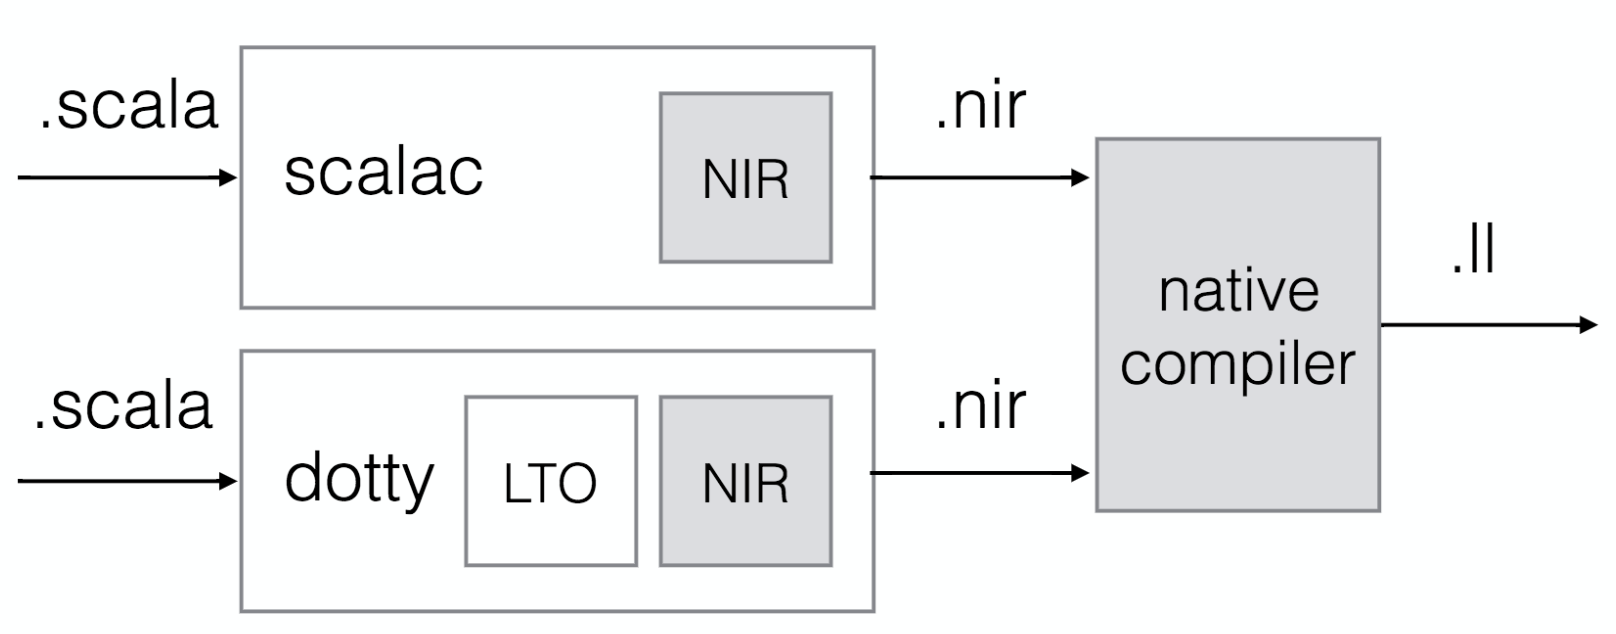
\includegraphics[width=5cm]{img/compilation.png}
\hspace{1cm}
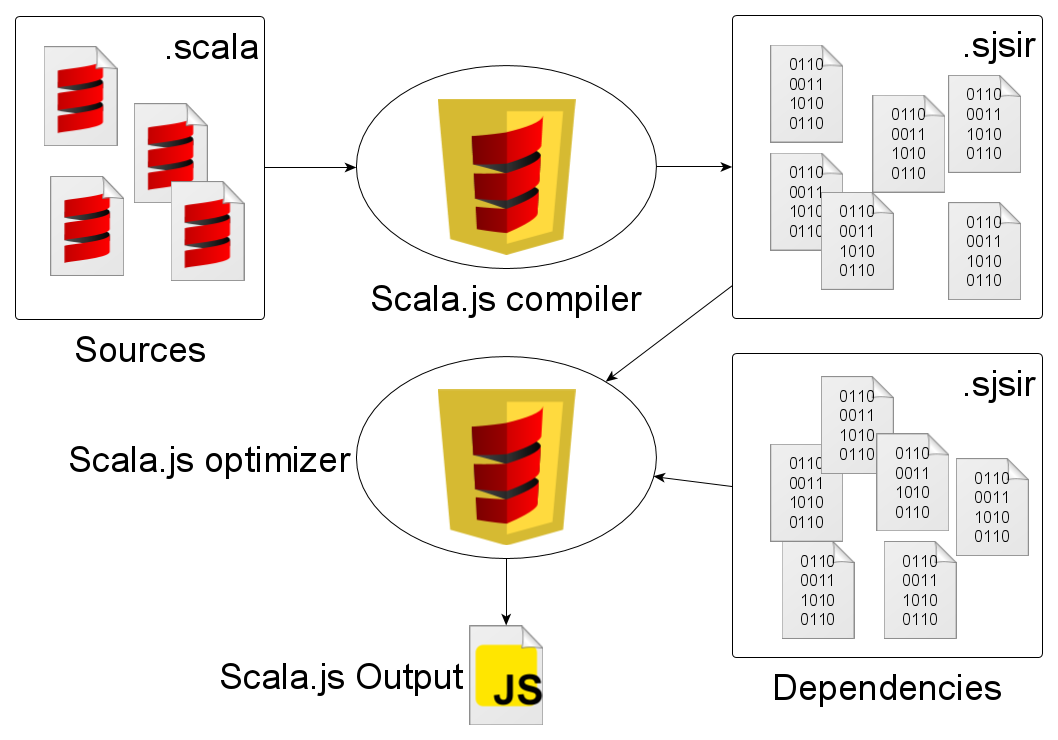
\includegraphics[width=5cm]{img/compilation-pipeline.png}
\end{frame}
\begin{frame}{Caveats}
	\begin{itemize}
		\item In pure cross Scala projects, you \bold{can't} use the JVM ecosystem (e.g. Thread?)...
  	\begin{itemize} 
				\item ... unless you build ad-hoc facades \href{http://www.scala-js.org/contribute/javalib.html}{\faLink}
				\item Several reimplemented APIs already exist \href{https://github.com/cquiroz/scala-java-time}{\faLink}
		\end{itemize}
		\item Javascript \& native libraries can be used \bold{only} in the corresponding runtime (in JVM you still cannot use JS libraries)
  	\item For using native \& JS libraries, you have to build ad-hoc facade (a là TypeScript with typings) \dots
   \begin{itemize}
		 \item For Scala.js an ScalablyTyped \href{https://scalablytyped.org/docs/readme.html}{\faLink} aims deriving Scala typing starting from TypeScript project 
	 \end{itemize} 
	 \item Application bundle size could be large since the code should include part runtime \& standard library
  \begin{itemize}
		\item Scala.js bundle could easily reach $\sim$ 1 Mb for the output file.
	\end{itemize}
	\end{itemize}
\end{frame}

\begin{frame}[fragile]{Scala.js \& Scala native configuration: SBT is your friend! \href{https://github.com/unibo-pps/scala-native-js-configuration}{\faLink}}
	\begin{itemize}
		\item Scalac does not natively produce JS \& Native .class
  	\item You have to enable \emph{plugins} via SBT configuration 
	\end{itemize}
	\begin{columns}
		\begin{column}[c]{0.5\textwidth}
			\begin{tcolorbox}[left=0pt, top=0pt, bottom=0pt, title=project/plugins.sbt]
				\begin{minted}{scala}
addSbtPlugin(
 "org.scala-js" % "sbt-scalajs" % "1.10.0"
)
// for native
addSbtPlugin(
 "org.scala-native" % "sbt-scala-native" % "0.4.4"
)
				\end{minted}
			\end{tcolorbox}
		\end{column}

		\begin{column}[c]{0.5\textwidth}
			\begin{tcolorbox}[left=0pt, top=0pt, bottom=0pt, title=build.sbt]
				\begin{minted}{scala}
enablePlugins(ScalaJSPlugin) // or ScalaNativePlugin
scalaVersion := "3.1.2"
// for JS
scalaJSUseMainModuleInitializer := true
				\end{minted}
			\end{tcolorbox}
		\end{column}
	\end{columns}
	
	\begin{itemize}
		\item ... still single platform
	\end{itemize}
\end{frame}
\begin{frame}[fragile]{Multi Platform Setup \href{https://github.com/unibo-pps/scala-cross-project}{\faLink}}
	\begin{itemize}
		\item Another SBT plugin to configure multiple platform projects: \bold{sbt-crossproject} \href{https://github.com/portable-scala/sbt-crossproject}{\faLink}
  	\item Enforce a project structure (configurable by different \emph{flavour})
		\begin{itemize}
			\item \texttt{CrossType.Pure}: pure cross-platform project (e.g. libraries), all code is placed in \texttt{/src}
   		\item \texttt{CrossType.Full}: project with platform-specific code (e.g. UI)
			\begin{itemize}
				\item \texttt{shared}: pure multi-platform code (e.g. data structure, interfaces, ...)
    		\item \texttt{js} and \texttt{jvm} and \texttt{native}: contain application platform-specific code (e.g. library usage, GUI, ...)
			\end{itemize}
		\end{itemize}
	\end{itemize}
	\begin{columns}
		\begin{column}[c]{0.5\textwidth}
			\begin{tcolorbox}[left=0pt, top=0pt, bottom=0pt, title=project/plugins.sbt]
				\begin{minted}{scala}

val crossOrg = "org.portable-scala"
val crossNative = "sbt-scala-native-crossproject"
val crossJs = "sbt-scalajs-crossproject"
addSbtPlugin(crossOrg % crossJs % "1.1.0")
addSbtPlugin(crossOrg % crossNative % "1.1.0")
addSbtPlugin(
	"org.scala-js" % "sbt-scalajs" % "1.10.0"
)
addSbtPlugin(
	"org.scala-native" % "sbt-scala-native" % "0.4.4"
)
				\end{minted}
			\end{tcolorbox}
		\end{column}

		\begin{column}[c]{0.5\textwidth}
			\begin{tcolorbox}[left=0pt, top=0pt, bottom=0pt, title=build.sbt]
				\begin{minted}{scala}
crossProject(JSPlatform, NativePlatform, JVMPlatform)
  .crossType(CrossType.Full) // or CrossType.Pure
// common settings, use %%% for cross library
	.settings(
		libraryDependencies ++= Seq(
      "org.scalatest" %%% "scalatest" % "3.2.12"
    )
	)
	.jsSettings()
	.nativeSettings()
	.jvmSettings() // standard "scala" world
				\end{minted}
			\end{tcolorbox}
		\end{column}
	\end{columns}
\end{frame}
%===============================================================================
\section{Project Examples}
%===============================================================================

\begin{frame}{Examples}
	\begin{alertblock}{Library Facade: Neaptic \href{https://github.com/unibo-pps/scala-js-facade-example}{\faLink}}
		\begin{itemize}
			\item You want to use a library that does not exist in the JVM ecosystem
   		\item You can use it unsafely (not recommended) or by \emph{creating a safe facade}
		\end{itemize}
	\end{alertblock}
	\begin{alertblock}{Cross-target Application: Winnig Four \href{https://github.com/unibo-pps/scala-cross-platform-winning-four}{\faLink}}
		\begin{itemize}
			\item You have an application logic written in pure scala (born for JVM)
			\item Then you want to share it in different platforms (e.g. Web, Android, ...)
   		\begin{enumerate}
				 \item Convert the project to a full cross-project
     		 \item Maintain the core logic in the shared part
         \item Create ad-hoc GUIs (or any specific platform code)
			 \end{enumerate} 
		\end{itemize}
	\end{alertblock}
	\begin{alertblock}{Full-Stack application: Todo Service \href{https://github.com/unibo-pps/scala-full-stack-app}{\faLink}}
		\begin{itemize}
			\item An application with a backend (JVM) and frontend (JS) part \faArrowRight \, classic Client-Server application
   		\item You have to maintain a shared part with data, services \& interfaces, \dots 
		\end{itemize}
	\end{alertblock}
\end{frame}

%===============================================================================
\section*{}
%===============================================================================

%/////////
\frame{\titlepage}
%/////////

%===============================================================================
\section*{\refname}
%===============================================================================

%%%%
\setbeamertemplate{page number in head/foot}{}
%/////////
\begin{frame}[c,noframenumbering, allowframebreaks]{\refname}
%\begin{frame}[t,allowframebreaks,noframenumbering]{\refname}
	\tiny
	\nocite{*}
	\printbibliography
\end{frame}
%/////////

%%%%%%%%%%%%%%%%%%%%%%%%%%%%%%%%%%%%%%%%%%%%%%%%%%%%%%%%%%%%%%%%%%%%%%%%%%%%%%%%
\end{document}
%%%%%%%%%%%%%%%%%%%%%%%%%%%%%%%%%%%%%%%%%%%%%%%%%%%%%%%%%%%%%%%%%%%%%%%%%%%%%%%%
